% chtex-lint: disable
\chapter{Menulis \LaTeX}

\section{Pengantar Penulisan \LaTeX}

Bagian ini memberikan pengenalan singkat penggunaan \LaTeX\ untuk penulisan ilmiah, meliputi penulisan teks tebal dan miring, pembuatan tabel, penyisipan gambar dengan sitasi, serta penulisan persamaan yang disertai sitasi. Contoh-contoh berikut dapat dijadikan acuan dasar dalam menulis dokumen tesis atau artikel ilmiah.

\subsection{Penulisan Teks Tebal dan Miring}

Penulisan teks tebal dan miring digunakan untuk menegaskan istilah tertentu atau memberi penekanan pada bagian penting.

\begin{itemize}
  \item Teks \textbf{tebal} menggunakan perintah \verb|\textbf{teks tebal}|.
  \item Teks \textit{miring} menggunakan perintah \verb|\textit{teks miring}|.
  \item Teks \emph{penekanan} menggunakan perintah \verb|\emph{teks penting}|.
\end{itemize}

Sebagai contoh: \textbf{istilah penting}, \textit{foreign term}, dan \emph{konsep utama} dapat digunakan untuk membedakan jenis penekanan dalam naskah.

\subsection{Penulisan Daftar (Itemize dan Enumerate)}

\LaTeX\ menyediakan beberapa lingkungan untuk membuat daftar. Dua yang paling umum digunakan adalah \verb|itemize| untuk daftar tanpa nomor (bullet points) dan \verb|enumerate| untuk daftar bernomor.

\textbf{Daftar Tanpa Nomor (Itemize)}

Gunakan lingkungan \verb|itemize| untuk membuat daftar dengan bullet:

\begin{verbatim}
\begin{itemize}
  \item Poin pertama
  \item Poin kedua
  \item Poin ketiga
\end{itemize}
\end{verbatim}

Hasil dari kode di atas:
\begin{itemize}
  \item Poin pertama yang menjelaskan konsep secara singkat.
  \item Poin kedua yang memberikan rincian atau contoh tambahan.
  \item Poin ketiga yang menegaskan hal-hal penting.
\end{itemize}

\textbf{Daftar Bernomor (Enumerate)}

Gunakan lingkungan \verb|enumerate| untuk membuat daftar dengan penomoran otomatis:

\begin{verbatim}
\begin{enumerate}
  \item Langkah pertama
  \item Langkah kedua
  \item Langkah ketiga
\end{enumerate}
\end{verbatim}

Hasil dari kode di atas:
\begin{enumerate}
  \item Langkah pertama dalam suatu prosedur atau tahapan analisis.
  \item Langkah kedua yang menjelaskan proses lanjutan.
  \item Langkah ketiga yang menggambarkan penyelesaian atau keluaran proses.
\end{enumerate}

\textbf{Daftar Bersarang (Nested List)}

Daftar dapat disarangkan hingga beberapa level:

\begin{enumerate}
  \item Kategori utama pertama
  \begin{enumerate}
    \item Sub-kategori 1.1
    \item Sub-kategori 1.2
  \end{enumerate}
  \item Kategori utama kedua
  \begin{itemize}
    \item Poin campuran dengan bullet
    \item Poin campuran lainnya
  \end{itemize}
\end{enumerate}

\subsection{Membuat Tabel dengan Format IEEE}

Tabel digunakan untuk menyajikan data secara terstruktur. Template ini menggunakan paket \texttt{booktabs} untuk menghasilkan garis horizontal berkualitas sesuai standar IEEE.

\textbf{Struktur Dasar Tabel}

Berikut adalah struktur dasar penulisan tabel:

\begin{verbatim}
\begin{table}[h]
  \centering
  \caption{Judul Tabel}
  \label{tab:label-tabel}
  \begin{tabular}{ccc}
    \toprule
    Kolom 1 & Kolom 2 & Kolom 3 \\
    \midrule
    Data 1  & Data 2  & Data 3 \\
    Data 4  & Data 5  & Data 6 \\
    \bottomrule
  \end{tabular}
\end{table}
\end{verbatim}

Perintah penting dalam format IEEE:
\begin{itemize}
  \item \verb|\toprule| -- garis horizontal tebal di atas tabel
  \item \verb|\midrule| -- garis horizontal tipis pemisah header dan data
  \item \verb|\bottomrule| -- garis horizontal tebal di bawah tabel
  \item \verb|\cmidrule{a-b}| -- garis horizontal parsial dari kolom a ke b
\end{itemize}

\textbf{Contoh Tabel Sederhana}

\begin{table}[h]
  \centering
  \caption{Contoh Tabel Sederhana dengan Format IEEE}
  \label{tab:contoh-tabel}
  \begin{tabular}{ccc}
    \toprule
    No & Parameter & Nilai \\
    \midrule
    1  & Contoh A & 0.85 \\
    2  & Contoh B & 0.90 \\
    3  & Contoh C & 0.78 \\
    \bottomrule
  \end{tabular}
\end{table}

\textbf{Contoh Tabel dengan Header Bertingkat}

\begin{table}[h]
  \centering
  \caption{Perbandingan Performa Model}
  \label{tab:performa-model}
  \begin{tabular}{lccc}
    \toprule
    \textbf{Model} & \textbf{Accuracy} & \textbf{Precision} & \textbf{Recall} \\
    \midrule
    Random Forest  & 0.92 & 0.89 & 0.91 \\
    SVM            & 0.88 & 0.85 & 0.87 \\
    Neural Network & 0.95 & 0.93 & 0.94 \\
    \midrule
    \textit{Rata-rata} & 0.92 & 0.89 & 0.91 \\
    \bottomrule
  \end{tabular}
\end{table}

Tabel \ref{tab:contoh-tabel} dan Tabel \ref{tab:performa-model} dapat dirujuk menggunakan perintah \verb|\ref{tab:label}|.

\subsection{Menyisipkan Gambar}

Gambar disisipkan menggunakan lingkungan \verb|figure| dengan perintah \verb|\includegraphics| dari paket \texttt{graphicx}.

\textbf{Struktur Dasar Gambar}

\begin{verbatim}
\begin{figure}[h]
  \centering
  \includegraphics[width=0.8\textwidth]{path/ke/gambar.png}
  \caption{Keterangan gambar.}
  \label{fig:label-gambar}
\end{figure}
\end{verbatim}

Opsi pengaturan ukuran gambar:
\begin{itemize}
  \item \verb|width=0.8\textwidth| -- lebar 80\% dari lebar teks
  \item \verb|height=5cm| -- tinggi tetap 5 cm
  \item \verb|scale=0.5| -- skala 50\% dari ukuran asli
  \item \verb|width=\linewidth| -- lebar penuh satu baris
\end{itemize}

\textbf{Contoh Penyisipan Gambar}

\begin{figure}[h]
  \centering
  \includegraphics[width=0.6\textwidth]{documents/Iris_dataset.png}
  \caption{Contoh dataset Iris yang diadaptasi dari penelitian sebelumnya \cite{Zhou2025}.}
  \label{fig:contoh-gambar}
\end{figure}

Gambar~\ref{fig:contoh-gambar} menunjukkan struktur dataset Iris yang umum digunakan dalam penelitian machine learning. Gunakan \verb|Gambar~\ref{fig:label}| untuk merujuk gambar (tanda \verb|~| mencegah pemisahan baris).

\textbf{Opsi Penempatan Float}

Opsi penempatan dalam tanda kurung siku:
\begin{itemize}
  \item \verb|[h]| -- here, tempatkan di posisi saat ini jika memungkinkan
  \item \verb|[t]| -- top, tempatkan di bagian atas halaman
  \item \verb|[b]| -- bottom, tempatkan di bagian bawah halaman
  \item \verb|[p]| -- page, tempatkan di halaman khusus float
  \item \verb|[H]| -- memaksa penempatan tepat di posisi kode (memerlukan paket \texttt{float})
  \item \verb|[htbp]| -- kombinasi, biarkan \LaTeX\ memilih yang terbaik
\end{itemize}

\subsection{Menulis Persamaan}

Persamaan matematika dapat ditulis dalam mode \emph{display} menggunakan lingkungan \verb|equation| dan diberi label untuk dirujuk kembali.

\textbf{Persamaan dengan Penomoran}

\begin{verbatim}
\begin{equation}
  y = f(x) = ax^{2} + bx + c
  \label{eq:persamaan-kuadrat}
\end{equation}
\myequations{Deskripsi Persamaan}
\end{verbatim}

Contoh hasil:

\begin{equation}
  y = f(x) = ax^{2} + bx + c
  \label{eq:persamaan-kuadrat}
\end{equation}
\myequations{Persamaan Fungsi Kuadrat}

Persamaan \eqref{eq:persamaan-kuadrat} dapat dirujuk menggunakan \verb|\eqref{eq:label}| atau \verb|\ref{eq:label}|. Perintah \verb|\myequations{...}| digunakan untuk menambahkan persamaan ke Daftar Persamaan.

\textbf{Persamaan Tanpa Penomoran}

Untuk persamaan yang tidak perlu dirujuk, gunakan \verb|\[ ... \]|:

\[
  \nabla J(\theta) = \frac{\partial J(\theta)}{\partial \theta}
\]

\subsection{Sitasi dan Daftar Pustaka}

Sitasi dalam template ini menggunakan format IEEE dengan perintah \verb|\cite{key}|. Contoh: \verb|\cite{Zhou2025}| menghasilkan \cite{Zhou2025}.

Langkah kompilasi untuk memproses sitasi:
\begin{enumerate}
  \item \textbf{XeLaTeX} -- kompilasi pertama
  \item \textbf{Biber} -- memproses bibliografi
  \item \textbf{XeLaTeX} -- kompilasi kedua dan ketiga
\end{enumerate}

\subsection{Label dan Rujukan Silang}

Gunakan \verb|\label{...}| untuk memberi penanda pada elemen, lalu rujuk dengan \verb|\ref{...}| atau \verb|\cref{...}|.

\begin{table}[h]
  \centering
  \caption{Konvensi Penamaan Label}
  \label{tab:konvensi-label}
  \begin{tabular}{lll}
    \toprule
    \textbf{Elemen} & \textbf{Prefix} & \textbf{Contoh} \\
    \midrule
    Gambar    & \texttt{fig:} & \verb|\label{fig:arsitektur}| \\
    Tabel     & \texttt{tab:} & \verb|\label{tab:hasil}| \\
    Persamaan & \texttt{eq:}  & \verb|\label{eq:loss-function}| \\
    Algoritma & \texttt{alg:} & \verb|\label{alg:training}| \\
    Kode      & \texttt{lst:} & \verb|\label{lst:python-code}| \\
    \bottomrule
  \end{tabular}
\end{table}

\section{Membuat Diagram dengan TikZ}

Paket \texttt{TikZ} digunakan untuk membuat gambar vektor langsung di dalam dokumen \LaTeX, seperti diagram blok, flowchart, dan grafik.

\subsection{Diagram Alur (Flowchart)}

Berikut contoh flowchart sederhana:

\begin{figure}[h]
  \centering
  \begin{tikzpicture}[
    node distance=2cm,
    >=Stealth,
    box/.style={draw, rectangle, rounded corners, minimum width=3cm, minimum height=1cm, align=center}
  ]
    \node[box] (start) {Mulai};
    \node[box, below of=start] (process) {Proses};
    \node[box, below of=process] (end) {Selesai};

    \draw[->] (start) -- (process);
    \draw[->] (process) -- (end);
  \end{tikzpicture};
  \caption{Contoh diagram alur sederhana menggunakan TikZ.}
  \label{fig:tikz-flowchart}
\end{figure}

\subsection{Grafik Fungsi}

TikZ juga dapat menggambar grafik fungsi matematika:

\begin{figure}[h]
  \centering
  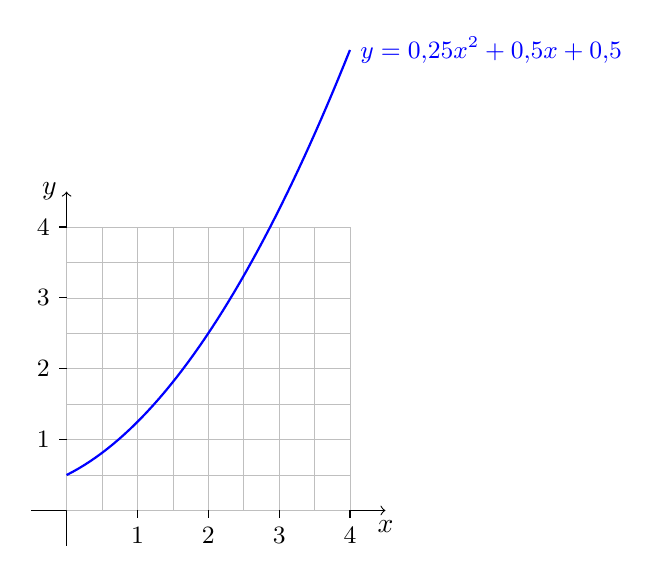
\begin{tikzpicture}[scale=0.9]
    \draw[->] (-0.5,0) -- (4.5,0) node[below] {$x$};
    \draw[->] (0,-0.5) -- (0,4.5) node[left] {$y$};
    \draw[help lines, step=0.5cm, lightgray] (0,0) grid (4,4);

    \foreach \x in {1,2,3,4}
      \draw (\x,0) -- (\x,-0.1) node[below] {\small \x};
    \foreach \y in {1,2,3,4}
      \draw (0,\y) -- (-0.1,\y) node[left] {\small \y};

    \draw[thick, blue, domain=0:4, samples=50]
      plot (\x, {0.25*\x*\x + 0.5*\x + 0.5})
      node[right] {\small $y = 0{,}25x^{2} + 0{,}5x + 0{,}5$};
  \end{tikzpicture}
  \caption{Contoh grafik fungsi kuadrat menggunakan TikZ.}
  \label{fig:tikz-grafik}
\end{figure}


\section{Menulis Pseudocode dan Algoritma}

Penulisan pseudocode atau algoritma dalam dokumen ilmiah berguna untuk menjelaskan langkah-langkah prosedur secara sistematis. Template ini menggunakan paket \texttt{algorithm2e} yang sudah dikonfigurasi di \verb|main.tex| dengan gaya penomoran per bab (misalnya Algoritma 2.1, 2.2, dst).

\subsection{Struktur Dasar Algoritma}

Berikut adalah struktur dasar penulisan algoritma menggunakan lingkungan \verb|algorithm|:

\begin{verbatim}
\begin{algorithm}[H]
  \caption{Nama Algoritma}
  \label{alg:label-algoritma}
  \KwInput{Deskripsi input}
  \KwOutput{Deskripsi output}

  langkah 1\;
  langkah 2\;
  \Return{hasil}\;
\end{algorithm}
\end{verbatim}

Perintah-perintah penting yang tersedia antara lain:
\begin{itemize}
  \item \verb|\KwInput{...}| -- untuk mendeskripsikan input algoritma.
  \item \verb|\KwOutput{...}| -- untuk mendeskripsikan output algoritma.
  \item \verb|\If{kondisi}{...}| -- untuk struktur kondisional \emph{if}.
  \item \verb|\eIf{kondisi}{...}{p...}| -- untuk struktur \emph{if-else}.
  \item \verb|\While{kondisi}{...}| -- untuk perulangan \emph{while}.
  \item \verb|\For{iterator}{...}| -- untuk perulangan \emph{for}.
  \item \verb|\ForEach{item}{...}| -- untuk perulangan \emph{foreach}.
  \item \verb|\Return{...}| -- untuk mengembalikan nilai.
  \item \verb|\Comment{...}| -- untuk menambahkan komentar.
\end{itemize}

\subsection{Contoh Algoritma Sederhana}

Berikut adalah contoh algoritma pencarian linear sederhana:

\begin{algorithm}[H]
  \caption{Pencarian Linear}
  \label{alg:linear-search}
  \KwInput{Array $A$ dengan $n$ elemen, nilai target $x$}
  \KwOutput{Indeks elemen jika ditemukan, $-1$ jika tidak}

  \For{$i \leftarrow 0$ \KwTo $n-1$}{
    \If{$A[i] = x$}{
      \Return{$i$}\;
    }
  }
  \Return{$-1$}\;
\end{algorithm}

Algoritma \ref{alg:linear-search} menunjukkan proses pencarian linear yang memeriksa setiap elemen array secara berurutan hingga menemukan nilai target atau mencapai akhir array.

\subsection{Contoh Algoritma dengan Struktur Kompleks}

Berikut adalah contoh algoritma yang lebih kompleks dengan penggunaan \emph{if-else} dan komentar:

\begin{algorithm}[H]
  \caption{Binary Search}
  \label{alg:binary-search}
  \KwInput{Array terurut $A$ dengan $n$ elemen, nilai target $x$}
  \KwOutput{Indeks elemen jika ditemukan, $-1$ jika tidak}

  $low \leftarrow 0$\;
  $high \leftarrow n - 1$\;

  \While{$low \leq high$}{
    $mid \leftarrow \lfloor (low + high) / 2 \rfloor$\; \Comment{Hitung indeks tengah}

    \eIf{$A[mid] = x$}{
      \Return{$mid$}\; \Comment{Elemen ditemukan}
    }{
      \eIf{$A[mid] < x$}{
        $low \leftarrow mid + 1$\; \Comment{Cari di bagian kanan}
      }{
        $high \leftarrow mid - 1$\; \Comment{Cari di bagian kiri}
      }
    }
  }

  \Return{$-1$}\; \Comment{Elemen tidak ditemukan}

\end{algorithm}

Algoritma \ref{alg:binary-search} menerapkan teknik \emph{divide and conquer} dengan kompleksitas waktu $O(\log n)$, yang jauh lebih efisien dibandingkan pencarian linear pada array berukuran besar.

\subsection{Merujuk Algoritma dalam Teks}

Untuk merujuk algoritma di dalam teks, gunakan perintah \verb|\ref{alg:label}| atau \verb|\cref{alg:label}|. Contoh:
\begin{itemize}
  \item \verb|Algoritma \ref{alg:binary-search}| menghasilkan: Algoritma \ref{alg:binary-search}
  \item \verb|\cref{alg:binary-search}| menghasilkan: \cref{alg:binary-search}
\end{itemize}

Dengan menggunakan paket \texttt{algorithm2e}, penulis dapat menyajikan algoritma secara profesional dan konsisten dengan format dokumen ilmiah.

\section{Menulis Kode Sumber dengan Syntax Highlighting}

Untuk menampilkan kode sumber dengan pewarnaan sintaks (\emph{syntax highlighting}), template ini menggunakan paket \texttt{listings} yang sudah dikonfigurasi di \verb|main.tex|. Paket ini mendukung berbagai bahasa pemrograman seperti Python, JavaScript, Java, C++, dan banyak lagi.

\subsection{Struktur Dasar Penulisan Kode}

Berikut adalah struktur dasar untuk menampilkan kode dengan caption dan label:

\begin{verbatim}
\begin{lstlisting}[style=pythonstyle, caption={Deskripsi Kode}, label={lst:label-kode}]
# kode program di sini
print("Hello, World!")
\end{lstlisting}
\end{verbatim}

Style yang tersedia antara lain:
\begin{itemize}
  \item \verb|pythonstyle| -- untuk bahasa Python
  \item \verb|javascriptstyle| -- untuk bahasa JavaScript
  \item \verb|javastyle| -- untuk bahasa Java
  \item \verb|defaultstyle| -- style umum untuk bahasa lainnya
\end{itemize}

\subsection{Contoh Kode Python}

Berikut adalah contoh kode Python dengan syntax highlighting:

\begin{lstlisting}[style=pythonstyle, caption={Contoh Fungsi Python untuk Menghitung Faktorial}, label={lst:python-factorial}]
def factorial(n):
    """
    Menghitung faktorial dari bilangan bulat non-negatif.

    Args:
        n: Bilangan bulat non-negatif
    Returns:
        Hasil faktorial dari n
    """
    if n < 0:
        raise ValueError("Input harus bilangan non-negatif")
    elif n == 0 or n == 1:
        return 1
    else:
        result = 1
        for i in range(2, n + 1):
            result *= i
        return result

# Contoh penggunaan
print(f"5! = {factorial(5)}")  # Output: 5! = 120
\end{lstlisting}

Kode \ref{lst:python-factorial} menunjukkan implementasi fungsi faktorial dalam Python dengan dokumentasi lengkap dan penanganan kesalahan.

\subsection{Contoh Kode JavaScript}

Berikut adalah contoh kode JavaScript:

\begin{lstlisting}[style=javascriptstyle, caption={Contoh Fungsi Async JavaScript}, label={lst:js-async}]
// Fungsi async untuk mengambil data dari API
async function fetchUserData(userId) {
    try {
        const response = await fetch(`/api/users/${userId}`);

        if (!response.ok) {
            throw new Error('User not found');
        }

        const userData = await response.json();
        return userData;
    } catch (error) {
        console.error('Error fetching user:', error.message);
        return null;
    }
}

// Contoh penggunaan
const user = await fetchUserData(123);
console.log(user.name);
\end{lstlisting}

\subsection{Contoh Kode Java}

Berikut adalah contoh kode Java:

\begin{lstlisting}[style=javastyle, caption={Contoh Class Java Sederhana}, label={lst:java-class}]
public class Calculator {
    private int result;

    public Calculator() {
        this.result = 0;
    }

    public int add(int a, int b) {
        result = a + b;
        return result;
    }

    public int subtract(int a, int b) {
        result = a - b;
        return result;
    }

    public static void main(String[] args) {
        Calculator calc = new Calculator();
        System.out.println("5 + 3 = " + calc.add(5, 3));
        System.out.println("5 - 3 = " + calc.subtract(5, 3));
    }
}
\end{lstlisting}

\subsection{Kode Inline dalam Teks}

Untuk menampilkan kode pendek di dalam paragraf, gunakan perintah \verb|\lstinline|. Contoh:

\begin{itemize}
  \item \verb|\lstinline{print("Hello")}| menghasilkan: \lstinline{print("Hello")}
  \item \verb|\lstinline[style=pythonstyle]{def main():}| menghasilkan: \lstinline[style=pythonstyle]{def main():}
\end{itemize}

\subsection{Merujuk Kode dalam Teks}

Untuk merujuk kode di dalam teks, gunakan perintah \verb|\ref{lst:label}|. Contoh:
\begin{itemize}
  \item \verb|Kode \ref{lst:python-factorial}| menghasilkan: Kode \ref{lst:python-factorial}
  \item \verb|Kode \ref{lst:js-async}| menghasilkan: Kode \ref{lst:js-async}
\end{itemize}

\subsection{Kustomisasi Tambahan}

Anda juga dapat mengkustomisasi tampilan kode secara langsung dengan opsi tambahan:

\begin{verbatim}
\begin{lstlisting}[
    language=Python,
    numbers=none,          % tanpa nomor baris
    frame=none,            % tanpa border
    backgroundcolor=\color{white}  % latar putih
]
# kode tanpa nomor baris dan border
x = 10
\end{lstlisting}
\end{verbatim}

Dengan paket \texttt{listings}, penulis dapat menyajikan kode sumber secara profesional dengan pewarnaan sintaks yang memudahkan pembaca memahami struktur dan logika program.
